\section{Case 2 - Anders blir oversett }

\subsection{Situasjon}

 Landsbydag 9 gikk mot slutten, og vi nærmet oss det klokkeslettet hvor vi vanligvis begynner med våre personlige refleksjoner. Det hadde blitt en del prat den siste tiden før vi skulle påbegynne refleksjonene, så atmosfæren lå til rette for fast og løst prat. En hel arbeidsdag var snart omme, så skillet mellom faglig og personlig prat ble mindre og mindre. Klokka slo 16.00 og tiden for personlig refleksjon var kommet. Gruppa hadde tidligere bestemt seg for å begynne med dagens reflektering presis klokken 16.00, for å få nok tid før vi måtte dra hjem for dagen. Jonas, Håkon og Lars diskuterte fortsatt, mens Ali satt på PCen. Det var uvisst for Anders hva Ali så på. Det er en generell tillit i gruppa som bygger på at man jobber når tiden er avsatt til jobbing. Til tross for dette hører Anders at praten til Jonas, Håkon og Lars sklir bort fra det faglige. \\

\textit{"Vi har meldt oss på, men i fjor ble vi diskvalifisert, så det er usikkert om vi får lov i år."}{--Lars}\\

Lars trekker på smilebåndet, og forteller om hvordan hockeylaget han spiller for er litt røffe i kantene. De får kanskje ikke får spille i turnering i år. Jonas og Håkon flirer. Klokka har nå bikket fem over fire og Anders tenker at dersom vi skal følge det målet vi hadde satt tidligere på dagen, så må vi komme i gang med de personlige refleksjonene våre.\\

\textit{"Gutta, nå er klokka fem over fire. Skal vi begynne med dagens personlige refleksjoner eller?"}{--Anders}\\

Blikkene fra Lars, Håkon og Jonas vrir seg mot Anders, men hodene flytter seg ikke. Det som sies blir registrert, men kroppsspråket deres anerkjenner det ikke.\\

\textit{"Jo da, sant det Anders."}{--Jonas}\\


Det går ikke mange sekundene fra Jonas sa seg enig, til samtalen er igang igjen. Håkon var fortsatt nysgjerrig på hva som skjedde med hockeylaget til Lars året før, og Jonas ville gjerne høre det samme. Øynene til Ali glir ned igjen på skjermen, da han ikke virket helt ferdig med hva han holdt på med. Denne reaksjonen fra samtlige i gruppa gjorde Anders litt irritert, og han tenkte at han skulle gjøre et lite eksperiment. Anders tok opp refleksjonsboka si og begynte å skrive, samtidig som han skulle bemerke seg hvor lang tid det ville ta fra han begynte på det avtalte arbeidet, til resten fulgte etter. Først etter fem minutter har alle gruppemedlemmene påbegynt refleksjonsskrivingen. Dette synes Anders var for dårlig, og valgte å ta det opp mot slutten av dagen.


\newpage


\subsection{Refleksjoner}

Etter å ha diskutert situasjonen i ettertid har det kommet frem forskjeller i hvordan man tolker både det som blir sagt og måten man legger fram argumentene på. Anders følte han tydelig uttrykket hva han ønsket gruppen skulle gjøre, men på en lite autoritær måte. Grunnen til at han ikke ønsket å være autoritær var fordi gruppa hadde en flat lederstruktur uten en utpekt leder. Han tror at grunnen til at beskjeden ikke ble tatt på alvor var fordi gruppa ikke kjente hverandre godt nok enda. Derfor er det vanskelig å vite hvor alvorlig et slikt ledende spørsmål blir mottatt. Selv om situasjonen oppstod halvveis ut i semesteret så mente Anders at det var for tidlig til at gruppa klarte å plukke opp signalene og væremåten til hverandre, på en måte hvor man faktisk forstod hva man mente. Gruppa kjente hverandre for dårlig til at en subtil beskjed skulle oppfattes som en "kommando". Nettopp av denne grunn ønsket ikke Anders å framstå som en autoritær type. Dette var grunnen til at han prøvde å få gruppa til å gjøre noe med kun et spørsmål.\\

Jonas og Ali følte det motsatte av Anders. De mente de kjente gruppa godt nok på dette tidspunktet til at de følte seg avslappet. Derfor trengte de ikke å følge med på slike signaler like mye som de gjorde i begynnelsen av semesteret. 
Lars satt med en oppfatning av situasjonen som en blanding av de to overnevnte. Han mente vi hadde blitt såpass kjent med hverandre at man føler seg komfortabel nok til ikke å holde fokus på å tolke signaler hele tiden, men samtidig ikke komfortabel nok til å skjære gjennom med ting. 
Det ble derfor en missforståelse i gruppa. Anders følte han hadde uttrykket seg klart og tydelig og følte seg derfor ignorert over at han ikke ble hørt mens resten av gruppa ikke hadde oppfattet situasjonen på den samme måte. \\

Denne situasjonen har fått Håkon til å tenke på hvor seriøst gruppa tar seg selv. Når gruppa mer eller mindre har blitt enige om å skrive refleksjoner klokka 16, men kollektivt bryter det løftet til fordel for uviktig prat, stiller han spørsmål ved hvor seriøst vi tok dette løftet til å begynne med. Når gruppa reflekterer rundt dette i ettertid, stiller Håkon spørsmål til akkurat hva det er som gjør at vi sier vi skal gjøre en ting, men ender opp med å gjøre noe annet. Hans tanke er at de fleste i gruppa setter det å hygge seg høyere enn jobbe med prosjektet til avtalt tid. Dette mener han strider med hva vi som gruppe har blitt enige om tidligere, og med hva hvert enkelt medlem har sagt de anser som viktig. Alle i gruppa har tidligere sagt at vi må ta det vi blir enig om å gjøre seriøst. Likevel har det dannet seg en slags kollektiv forståelse for hvordan man forholder seg til hverandre og oppgavene, som nesten alle i gruppa deler og som ikke stemmer overens med hva vi har avtalt.\\

Lars tror at vi ikke bare bryter tidligere avtaler for egen hygge. Han mener at det er svært viktig for sluttproduktet at gruppa har god kjemi og trivsel, og at det derfor skal være rom for snakk utenom det faglige. Alle sier seg enig i dette, men spørsmålet er i hvilken grad. Skal trivsel alltid trumfe arbeid, eller bare av og til? Lars trodde at det i denne situasjonen resulterte i at folk var slitne og at det var da helt vanlig menneskelig atferd å fokusere på å more seg selv i større grad. Mulighetene for frustrasjon når man er sliten er langt høyere, og tilbøyeligheten for å hygge seg er større. Dermed mener Lars at det ville være mest konstruktivt for gruppas helhetlige framgang å prioritere trivselen mot slutten av dagen. \\

Håkon kjøper ikke helt dette, og mener heller at vi bare skyr arbeid når vi er slitne og at fokuset på hygge er mer en distraksjon enn noe konstruktivt. Han tror ikke dette har videre positiv innvirkning på sluttproduktets resultat. Dette mener Lars blir litt feil, siden trivsel er en viktig nøkkel for prestasjonen vår. Anders kommenterer at dette virker som en vanskelig balansegang. Fra artikkelen "Promote an Appropriate Ratio of Task and Supportive Communications" i EiT-kompendiet \cite{groupEfficiencyModel}, sies det at de mest effektive gruppene bruker omlag 70-80\% av all sin kommunikasjon på temaer relatert til oppgaver og mål. Her brukes eksempelet om at dersom man diskuterer en fotballkamp i en lengre periode, bør man flytte fokus tilbake til arbeidet. Men, dersom det har blitt jobbet intenst i en lengre periode, bør det belønnes med litt vilkårlig løst prat for trivselens skyld. \\

Det kom fram i gruppereflektering at denne situasjonen også er litt knyttet til en annen splittelse innad i gruppa som gjelder tidsbruk. Anders syntes ikke det var poeng i å sitte til kl 17.00, bare for å sitte til kl 17.00, selv om det var dette som ble bestemt å være den faste arbeidstiden. I stedet for å sitte en halvtime og prate om sosiale ting kunne Anders heller ha tenkt seg å dra hjem. Han har nemlig fast avtale på onsdager kl 17.00 om felles middag i kollektivet han bor i. Anders har et ønske om å være hjemme til denne tiden, men føler ikke at det er en god nok grunn til å framskynde arbeidet i gruppa slik at han kommer hjem til dette tidspunktet. Han synes personlige preferanser er underordnet arbeidsavtalen gruppa har laget.\\

Dette var enda en grunn til at han prøvde å subtilt påvirke gruppa slik at gruppa blir ferdige før 17, men kun dersom det var ikke-faglig snakk. De andre gruppemedlemmene vet at Anders har denne avtalen og det har tidligere vært en diskusjon rundt dette. Der kom det fram at gruppa mente arbeidstiden var viktigere enn at han skulle rekke en middagsavtale som stridet med arbeidstiden. Anders var originalt enig i dette, og det førte da kanskje til at han ikke var like bestemt når han foreslo at vi skulle begynne refleksjonsskrivinga. Når gruppa reflekterer over dette i ettertid, kommer det fram at det var litt synd at gruppa stod så hardt på at hans middagavtaler skulle vike for arbeidstiden, når denne arbeidstiden ble brukt til uviktig snakk.
\\
%- 1) Anders følte han var tydelig i hva han ønsket at gruppa skulle gjøre, men det ble ikke oppfattet som tydelig av de andre i gruppa.

%- 1) Anders tror det kan være for tidlig til å plukke opp signalene/væremåten til hverandre. Anders ønsker ikke å skjære gjennom enda. 

%- 2) Jonas og Ali tror litt det motsatte, hvor de føler seg såppass avslappet at de ikke følger meg like sterkt på signaler fra andre.

%- 3) Lars tror det kan være et grenseskille mellom de to overnevnte situasjonene, hvor man føler seg komfortabel nok til å ikke være obs hele tiden, men ikke komfortabel nok til å skjære gjennom med ting.

%- Anders har følt seg oversett litt tidligere, og det har kanskje underbygget en følelse som boblet litt opp til denne situasjonen.

%- 4) Håkon setter spørsmål ved gruppas integritet til seg selv. Tar vi oss på alvor når vi setter en frist men ikke følger den? Anders tror vi kanskje prioriterer trivsel høyere enn framgang i prosjektet. Lars tror det er viktig å ha fokus på trivsel for å gjøre et godt prosjekt.

%- 4) Anders synes det er en vanskelig situasjon å balansere mellom å la lite viktig prat bryte mellom prosjektets planer og framgang.

%- 5) Anders synes at sin grunn (å bli ferdig for å gå hjem og spise middag) kanskje ikke var viktig nok for å presse på.

%- 5) Anders synes at det ikke er noe vits i å sitte til 17 bare for å sitte til 17.

%- 6) Hvordan pushe folk til å jobbe uten å framstå kjip?


\newpage

\subsection{Aksjoner}

I starten av dette faget, rundt tiden vi dannet vår samarbeidskontrakt, så ble gruppa enig i at når noen snakker så skal man legge fra seg alt annet og følge med. Man skulle følge såpass med at man tok til seg det som ble sagt og skulle kunne svare konstruktivt på det, dersom man hadde innspill. Når forslaget til Anders om å starte dagens personlige refleksjonsskriving så vidt blir anerkjent, kan det tyde på at her innfridde ikke resten av gruppa godt nok på dette punktet. Det er vanskelig å innordne seg til slik man avtaler at man skal oppføre seg. Dette gjelder spesielt når man begynner å bli sliten i hodet etter en lang dag. Likevel er det et punkt gruppa mener er svært viktig for at alle skal føle seg inkludert, og ser dermed på dette som noe som bør jobbes kontinuerlig med å etterstrebe så bra man klarer.\\
\\

Under landsbydag 3 hadde vi en øvelse som het "ta plass, gi plass", der vi skulle visualisere hvor stor andel av taletiden og hvor stor del av rommet vi mente at hvert medlem tok. Det viste seg at alle i gruppa hadde omtrent det samme bilde på hvor mye plass hver enkelt tok. Det så omtrent ut som Figur \ref{fig:taplass}.

\begin{figure}[H] 
    \centering
    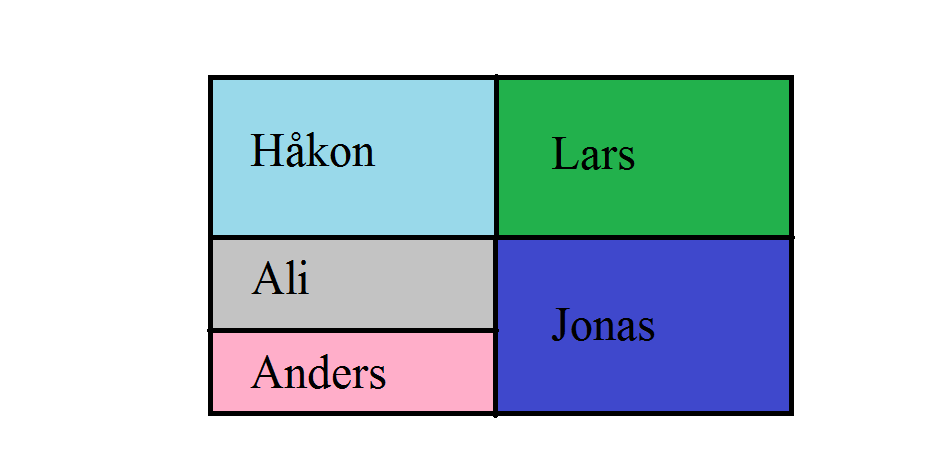
\includegraphics[scale=0.5]{images/taplass.png}
    \caption{Visuell framstilling av hvor mye plass hvert gruppemedlem tok}
    \label{fig:taplass}
\end{figure}\\


Ali og Anders tok ikke ordet like mye i starten. Når gruppa reflekterte rundt dette kom det fram at Anders var litt usikker på om hva han hadde å si var viktig nok til at det var behov for å si det. Det ble spekulert i om Anders ikke følte seg komfortabel nok med å si fra sterkt nok om hva han mener, i frykt for å si "noe dumt". Dette trodde Anders at kanskje resulterte i at han ufarliggjorde det han sa, og at gruppa kanskje ikke tok det like seriøst. Her mente Anders at et virkemiddel for å ikke bli oversett på det han sier, er at han må å være mer frampå og ta mer plass. På denne måten vil det minske risikoen for at hva han sier ikke blir anerkjent, og at Anders vil føle seg mer delaktig i bestemmelsene. Det vi i gruppa kom fram til at vil være en optimal balansegang for oss, er at personen som snakker må prøve å være bestemt i å få fram synspunktet sitt. Resten av gruppa må ha i bakhodet at det er viktig å være attentativ og respekterende ovenfor den som snakker for at alle skal føle seg komfortable og inkludert i gruppearbeidet.\\
\\

%- ta plass gi plass

%- de som tar mye plass er kanskje litt mer hensynsløs i snakkestilen.

%- sette fast klokkeslett og være mer obs på det.

%- Anders må tørre å være litt mer standhaftig (faglig innhold)

%- Andre må være litt mer obs

\newpage